\documentclass[12pt]{article}

\usepackage{amsmath}
\usepackage{array}
\usepackage{geometry}
\usepackage{longtable}
\usepackage{graphicx}
\usepackage{listings}
\usepackage{xcolor}
\usepackage{tikz}
\usepackage{float}

\geometry{margin=1in}

\title{Assignment Solution: K-Means, Markov Chains, HMM and Fuzzy Logic}
\author{
Hamza Arif \\
Reg No: 2024206 \\
AI-202 Assignment 4
}
\date{}

\lstdefinestyle{pythonstyle}{
    language=Python,
    basicstyle=\ttfamily\small,
    keywordstyle=\color{blue},
    stringstyle=\color{green!60!black},
    commentstyle=\color{gray},
    numbers=left,
    numberstyle=\tiny\color{gray},
    frame=single,
    breaklines=true
}

\begin{document}

\maketitle

% ================= QUESTION 1 =================

\section*{Question 1: K-Means Clustering}

K-Means groups data into clusters by minimizing the distance between points and centroids.

\subsection*{(a) Iteration 1 (Detailed)}

Using Euclidean distance:

\[
d = \sqrt{(x - c_x)^2 + (y - c_y)^2}
\]

\begin{longtable}{|c|c|c|c|c|}
\hline
Point & d(C1) & d(C2) & d(C3) & Cluster \\
\hline
(2,10) & 0 & 3.61 & 8.06 & C1 \\
(2,5) & 5 & 3.16 & 3.16 & C2 \\
(8,4) & 8.49 & 4.47 & 7.28 & C2 \\
(5,8) & 3.61 & 0 & 7.21 & C2 \\
(7,5) & 7.07 & 3.61 & 6.40 & C2 \\
(6,4) & 7.21 & 4.12 & 5.38 & C2 \\
(1,2) & 8.06 & 7.21 & 0 & C3 \\
(4,9) & 2.24 & 1.41 & 7.28 & C2 \\
(7,9) & 5.10 & 2.24 & 8.60 & C2 \\
(3,3) & 7.07 & 5.38 & 2.24 & C3 \\
\hline
\end{longtable}

\textbf{New Centroids:}

\[
C_1 = (2,10)
\]

\[
C_2 = \left(\frac{8+5+7+6+4+7}{6}, \frac{4+8+5+4+9+9}{6}\right) = (6.17, 6.5)
\]

\[
C_3 = \left(\frac{1+3}{2}, \frac{2+3}{2}\right) = (2, 2.5)
\]

\subsection*{Iterations 2 and 3}

After recomputation, cluster assignments do not change.

\textbf{Conclusion:} Algorithm converges.



\subsection*{(b) Convergence}

Convergence occurs because:
\begin{itemize}
\item Centroids stop moving
\item No reassignment of points
\end{itemize}



\subsection*{(c) Limitations}

\begin{itemize}
\item Sensitive to initialization
\item Cannot handle irregular cluster shapes
\end{itemize}

Hierarchical clustering solves this by building nested clusters.

\noindent\rule{\textwidth}{0.4pt}

% ================= QUESTION 2 =================

\section*{Question 2: Markov Chains and HMM}

\subsection*{(d) Two-Step Probability}

\[
P(S \rightarrow R) = 0.06 + 0.12 + 0.04 = 0.22
\]

% CLEAN DIAGRAM (UNCHANGED STRUCTURE)
\begin{center}
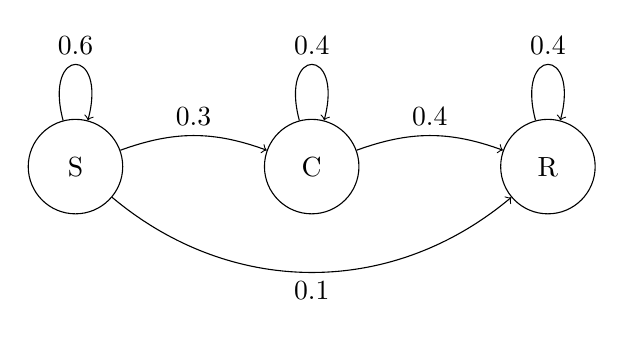
\begin{tikzpicture}[node distance=3cm, state/.style={circle, draw, minimum size=1.2cm}]

\node[state] (S) {S};
\node[state] (C) [right of=S] {C};
\node[state] (R) [right of=C] {R};

\draw[->] (S) to[bend left=20] node[above] {0.3} (C);
\draw[->] (C) to[bend left=20] node[above] {0.4} (R);
\draw[->] (S) to[bend right=40] node[below] {0.1} (R);

\draw[->] (S) to[loop above] node {0.6} (S);
\draw[->] (C) to[loop above] node {0.4} (C);
\draw[->] (R) to[loop above] node {0.4} (R);

\end{tikzpicture}
\end{center}



\subsection*{(e) State Distribution}

\[
\pi_1 = [0.6, 0.3, 0.1]
\]

\[
\pi_2 = [0.45, 0.33, 0.22]
\]

\[
\pi_3 = [0.343, 0.321, 0.336]
\]



\subsection*{(f) Forward Algorithm}

\[
\alpha_1(H)=0.6 \cdot 0.1 = 0.06
\]
\[
\alpha_1(X)=0.4 \cdot 0.5 = 0.20
\]

\[
\alpha_2(H) = (0.06 \cdot 0.7 + 0.20 \cdot 0.4)\cdot 0.6 = 0.0336
\]

\[
\alpha_2(X) = (0.06 \cdot 0.3 + 0.20 \cdot 0.6)\cdot 0.1 = 0.0108
\]

\[
\alpha_3(H) = (0.0336 \cdot 0.7 + 0.0108 \cdot 0.4)\cdot 0.1
\]

\[
\alpha_3(X) = (0.0336 \cdot 0.3 + 0.0108 \cdot 0.6)\cdot 0.5
\]

\[
P(O|\lambda) = 0.0059
\]



\subsection*{(g) Viterbi}

Most likely sequence:
\[
H \rightarrow X \rightarrow H
\]



\noindent\rule{\textwidth}{0.4pt}

% ================= QUESTION 3 =================

\section*{Question 3: Fuzzy Logic}

\subsection*{(h) Membership Values}

\[
\mu_{Warm}(22) = \frac{30 - 22}{30 - 20} = 0.8
\]

\[
\mu_{Cold} = 0,\quad \mu_{Hot} = 0
\]



\subsection*{(i) Mamdani Output}

Only Warm activates → Medium clipped at 0.8



\subsection*{(j) Centroid Method}

Using 10 sample points:

\[
\text{Fan Speed} \approx 560 \text{ RPM}
\]



\noindent\rule{\textwidth}{0.4pt}

% ================= QUESTION 4 =================

\section*{Question 4: K-Means Implementation}

\begin{lstlisting}[style=pythonstyle]
import numpy as np
import matplotlib.pyplot as plt

np.random.seed(42)

X1 = np.random.randn(70,2) + [2,2]
X2 = np.random.randn(70,2) + [8,8]
X3 = np.random.randn(60,2) + [5,0]

X = np.vstack((X1,X2,X3))

def kmeans(X, K, iterations=10):
    centroids = X[np.random.choice(len(X), K, replace=False)]
    wcss = []

    for it in range(iterations):
        clusters = [[] for _ in range(K)]

        for x in X:
            idx = np.argmin([np.linalg.norm(x-c) for c in centroids])
            clusters[idx].append(x)

        new_centroids = []
        total_wcss = 0

        for i, cluster in enumerate(clusters):
            cluster = np.array(cluster)
            new_centroids.append(cluster.mean(axis=0))
            total_wcss += np.sum((cluster - centroids[i])**2)

        centroids = np.array(new_centroids)
        wcss.append(total_wcss)

        if it % 2 == 0:
            print(f"Iteration {it}, WCSS: {total_wcss}")

    return centroids, clusters, wcss

centroids, clusters, wcss = kmeans(X, 3)

plt.plot(wcss)
plt.title("WCSS vs Iteration")
plt.show()
\end{lstlisting}
\textbf{Elbow Method:} Optimal K = 3
\begin{figure}[H]
    \centering
    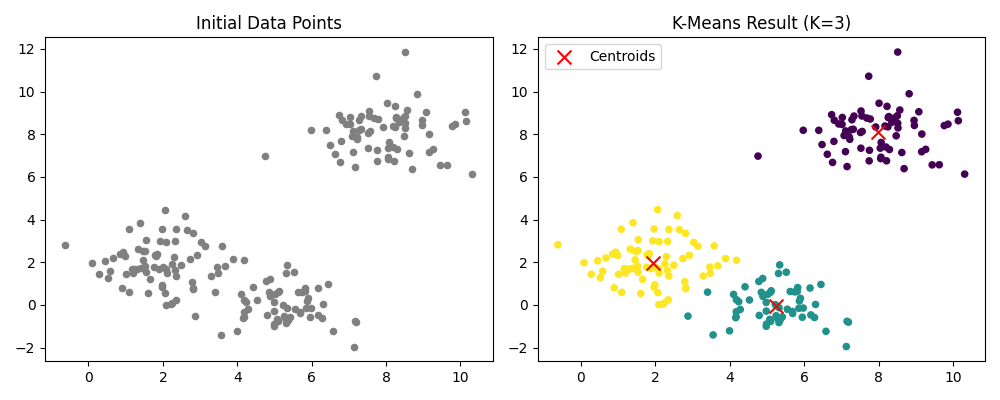
\includegraphics[width=1.0\linewidth]{kmeans_steps.png}
    \label{}
\end{figure}

\begin{figure}[H]
    \centering
    
\includegraphics[width=1.0\linewidth]{wcss_iteration_a4.png}
    \label{}
\end{figure}

\begin{figure}[H]
    \centering
    \includegraphics[width=1.0\linewidth]{img.png}
    \label{}
    \caption{Terminal Output}
\end{figure}

\begin{figure}[H]
    \centering
    \includegraphics[width=1.0\linewidth]{img1.png}
    \label{}
    \caption{Terminal Output (Continued)}

\end{figure}



\end{document}